Beyond the CCD approximation, we can also look at the CCDT-1 coupled-cluster approximation, adding some aspects of the $\hat{T}_3$ excitation operator into the calculations without the full-time needed for a complete CCDT calculation. In the next section, we will also consider the CCD(T) approximation, another coupled-cluster approximation that adds some aspects of the $\hat{T}_3$ operator into the calculations using a different algorithm.

First, we should verify that the CCDT-1 approximation with the same NNLO chiral potentials gives a different (and more accurate) approximation than the CCD approximation for pure neutron matter. In Fig. \ref{fig:ccd_vs_ccdt1}, the CCD correlation energies per particle are plotted as a function of the density of the pure neutron matter system for 66 neutrons and at densities around nuclear density with the solid red line. The CCD calculations shown were performed at 1,478 single-particle states, where the calculations converged. For the CCDT-1 calculations, shown with the solid black line, the calculations were also performed with the NNLO chiral potentials for pure neutron matter and 66 neutrons and at densities around nuclear density. As a result, the correlation energy calculations using CCDT-1 converge much faster than for CCD and only need 514 single-particle states to reach convergence. Additionally, since CCDT-1 calculations scale as $O(M^7)$ compared to a CCD calculation at $O(M^6)$, performing CCDT-1 calculation at higher values of M is computationally prohibitive. As shown in Fig \ref{fig:ccd_vs_ccdt1}, the CCD and CCDT-1 approximations give significantly different predictions for the correlation energies at each density value shown.

\begin{figure}
    \centering
    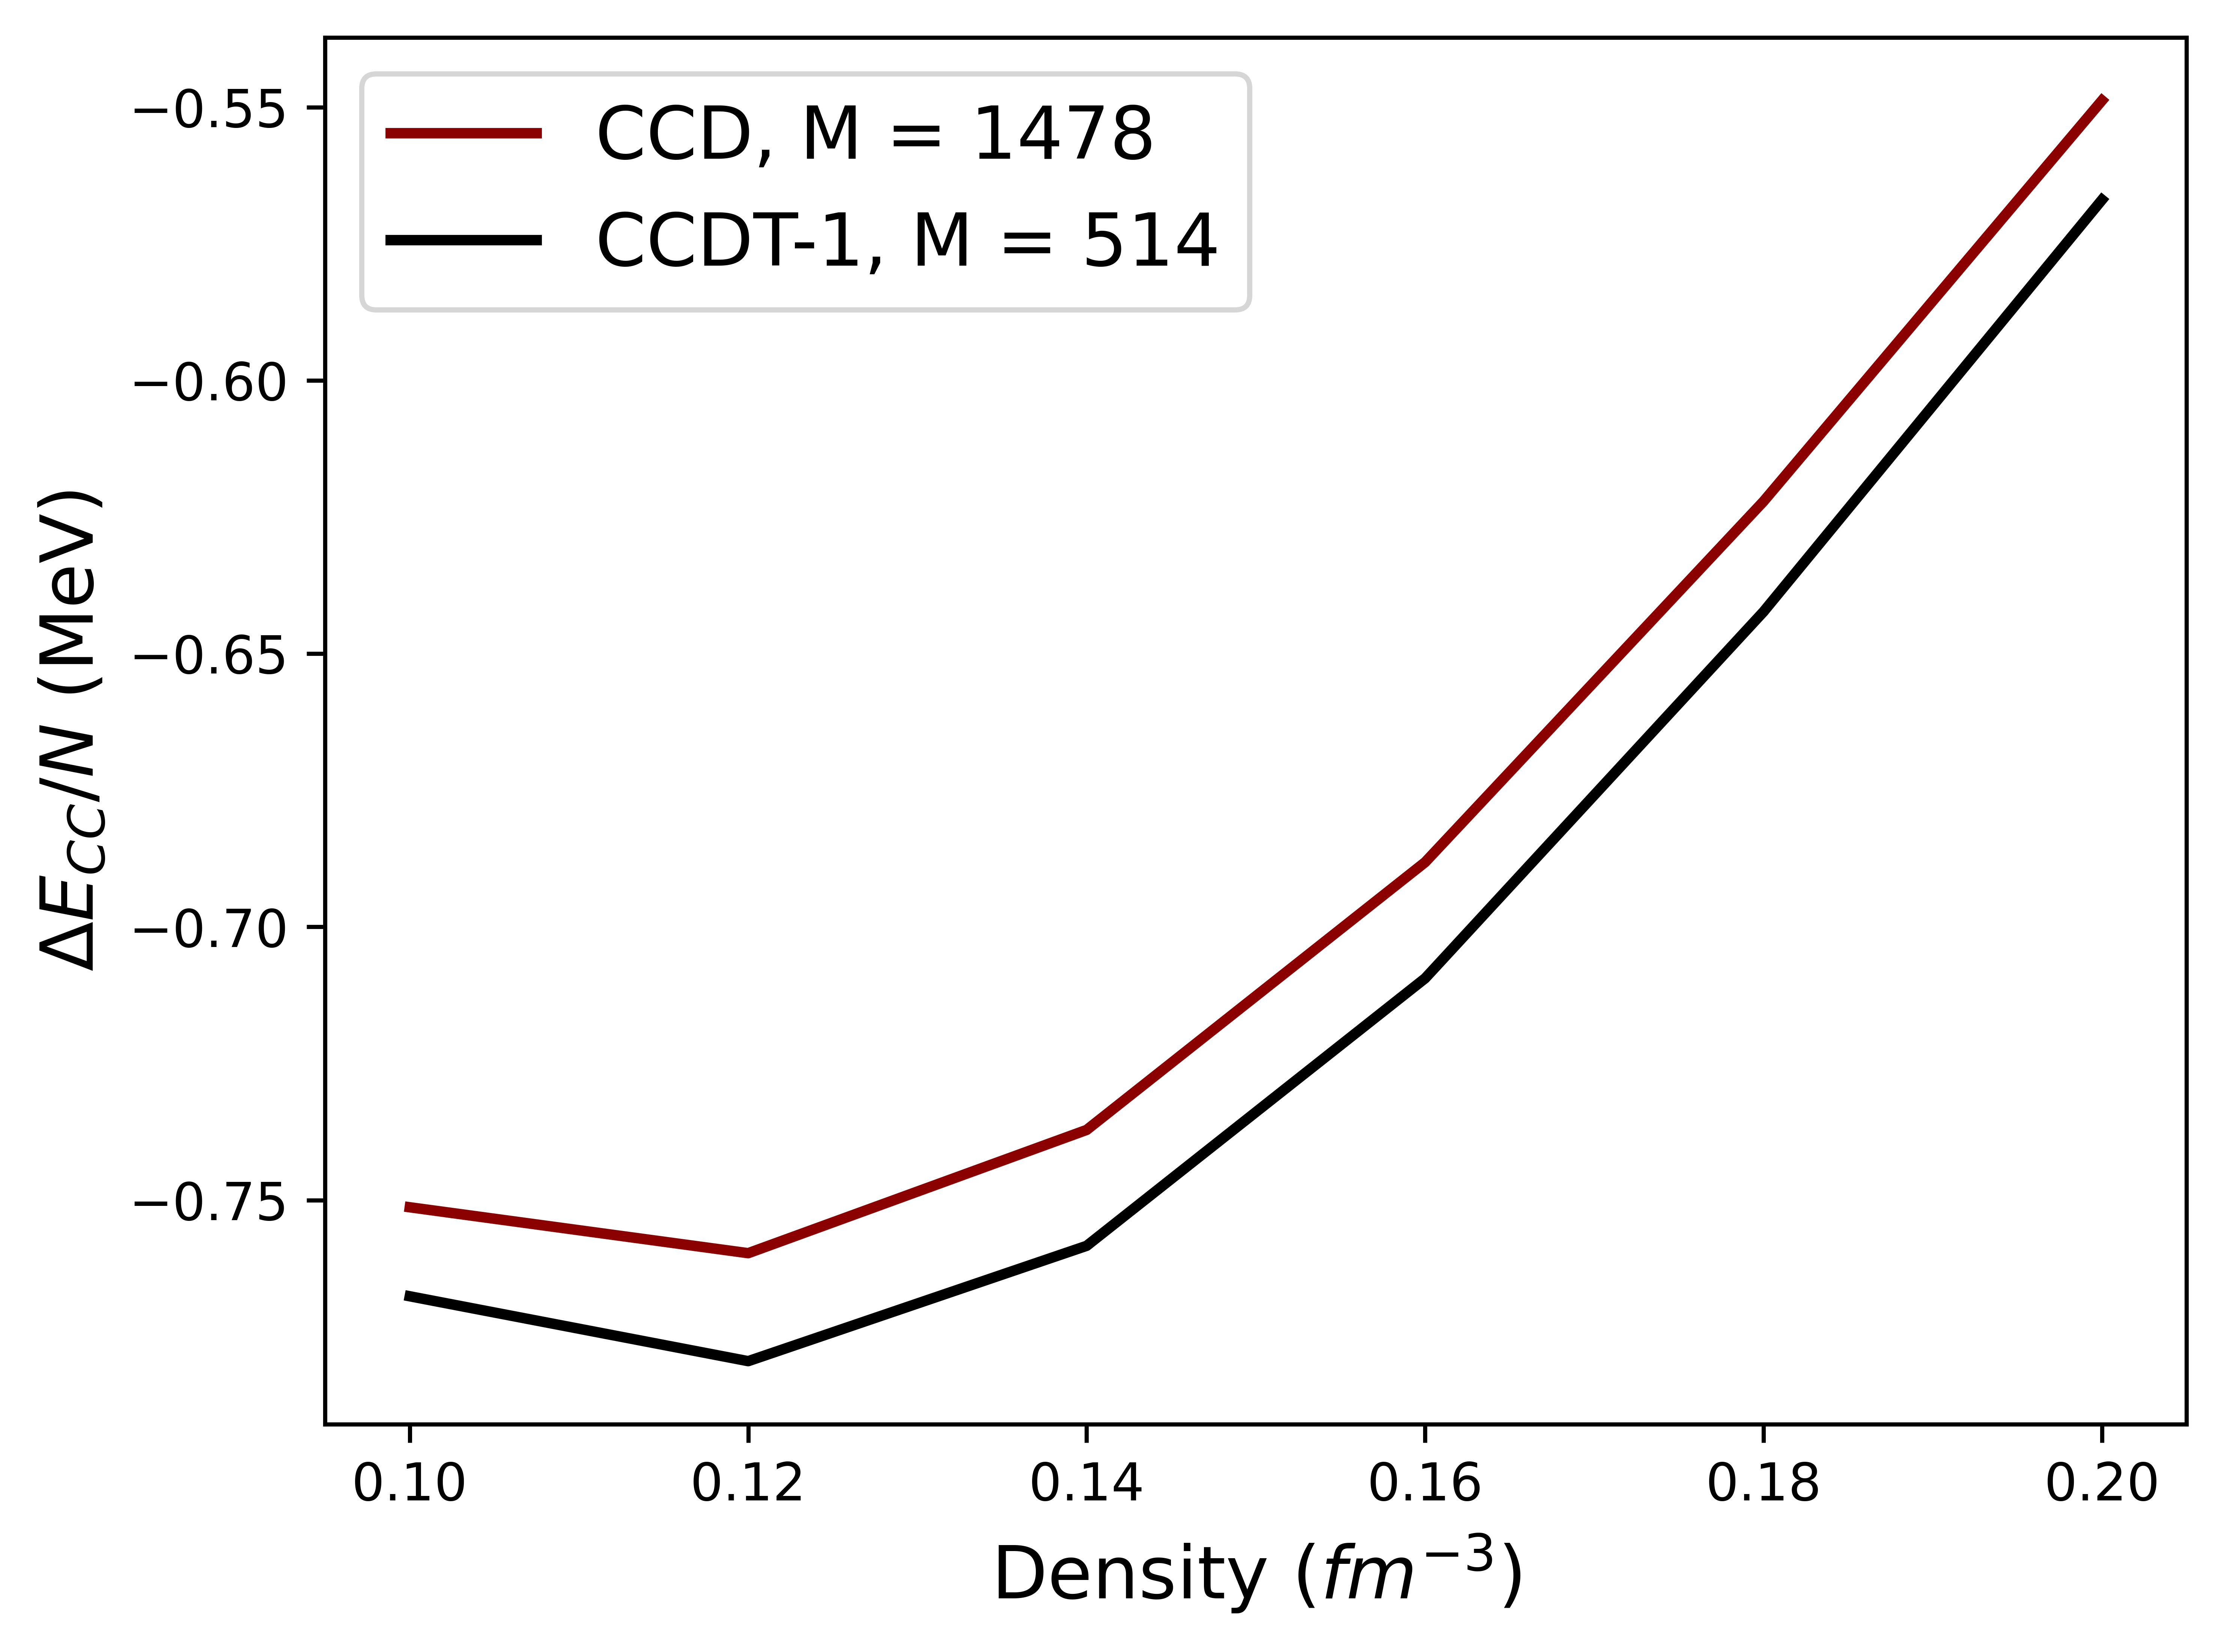
\includegraphics[scale=0.75]{Images/Chapter7/ORNL/ccdt1_nuclear_neutron_matter_no_ML.png}
    \caption{A comparison between the CCD and CCDT-1 correlation energies for a pure neutron matter system (N = 66 neutrons) with NNLO chiral potentials and for densities around nuclear density.  The CCDT-1 approximation consistently gives a lower correlation energy than CCD correlation energy at all densities in the graph.}
    \label{fig:ccd_vs_ccdt1}
\end{figure}

We can also compare the run times needed to complete a CCDT-1 calculation over a CCD calculation. Fig. \ref{fig:ccd_ccdt1_times} shows the total run time needed to complete a CCDT-1 calculation on Michigan State University's High-Performance Computing Center using Intel Xeon nodes with a clock speed of 2.4 GHz and 24 MPI nodes per run. The results in this figure were collected by performing CCDT-1 calculations on a pure neutron matter system with chiral NNLO potentials and with 66 neutrons and a density of 0.16 fm$^{-3}$. The results are reported in node hours. It is obvious that the run time increases very quickly with the number of single-particle states in the calculation. This rapid increase in run time is even more apparent if we plot the CCD and CCDT-1 run times on the same plot, as in Fig. \ref{fig:ccd_ccdt1_times}.  Though the CCDT-1 calculation converges at a smaller number of single-particle states, the total run time needed is drastically higher than that needed for the CCD calculations. At 514 single-particle states, the CCDT-1 calculation takes over 15 times longer than the CCD calculation at the same number of single-particle states. So even though we were motivated to use the SRE method to save time on the CCD calculations with the chiral NNLO potentials due to their run times, there is even more of a need for an accurate extrapolation method for the CCDT-1 calculations as their run times are an order of magnitude larger.

\begin{figure}
    \centering
    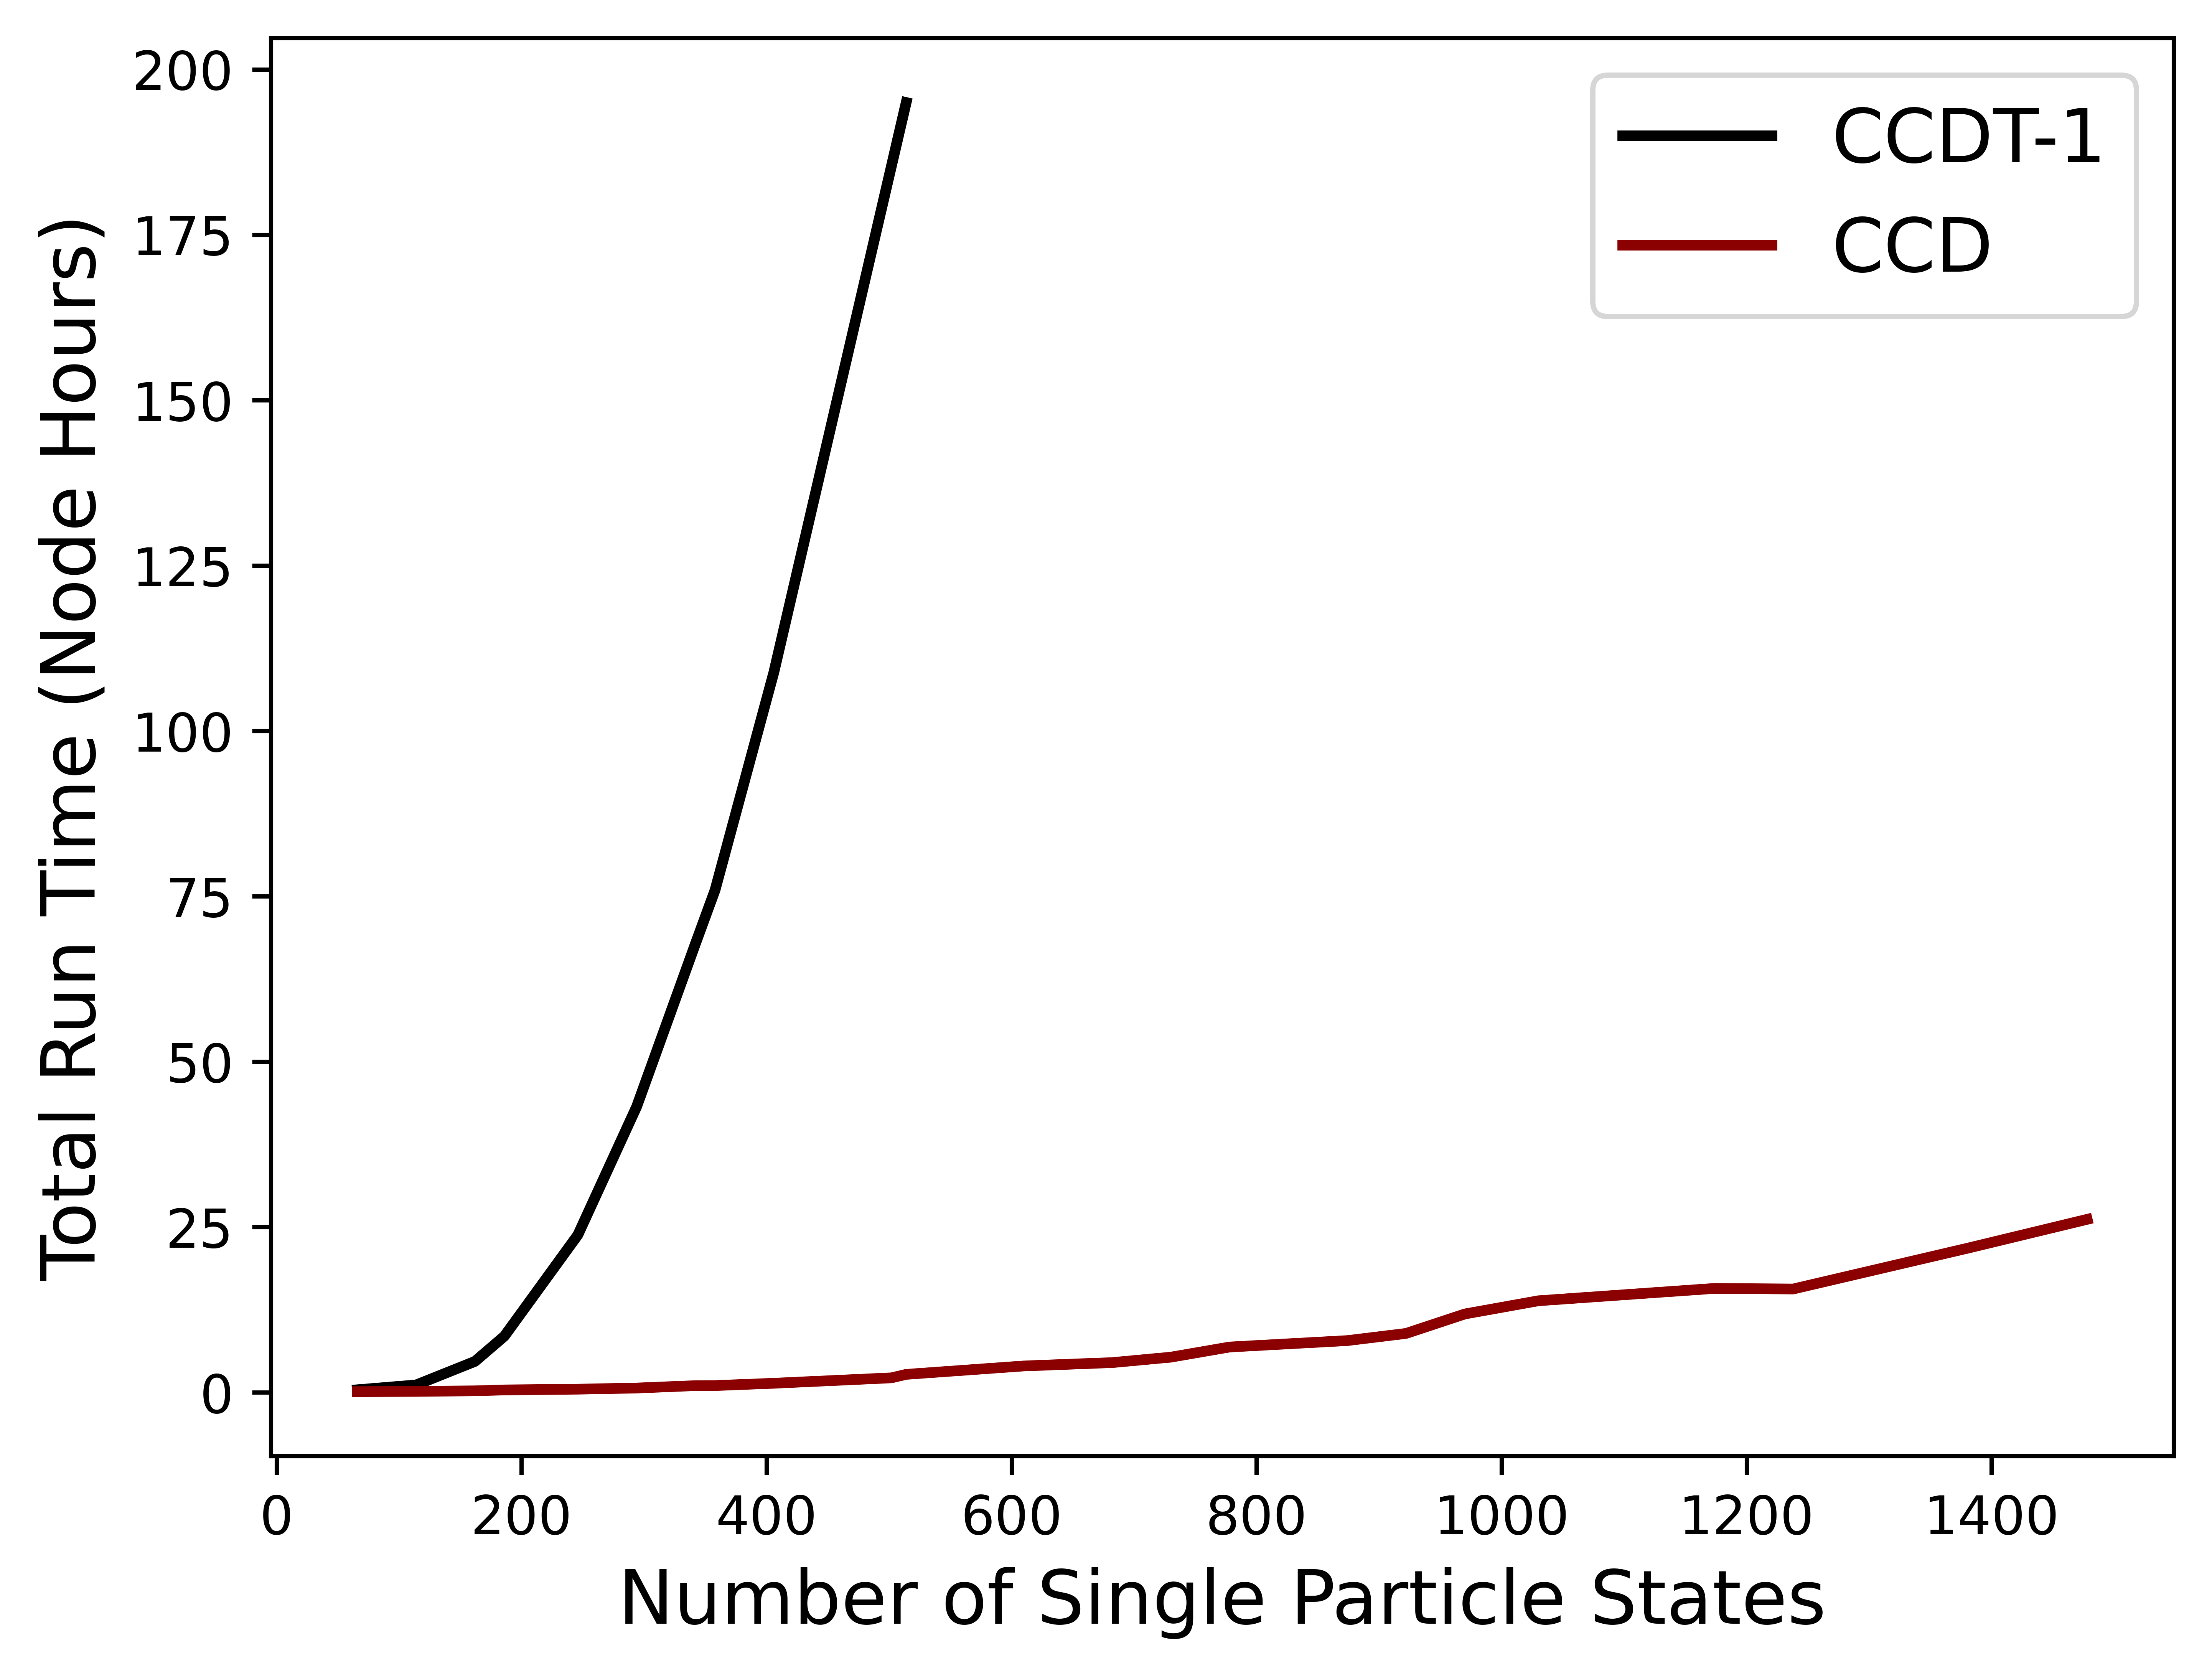
\includegraphics{Images/Chapter7/ORNL/ccdt1 and ccd times.png}
    \caption{The run times needed to complete CCD and CCDT-1 calculations for a PNM system reported in node hours.}
    \label{fig:ccd_ccdt1_times}
\end{figure}

Next, we will look at the feasibility of predicting the CCDT-1 correlation energy from the MBPT2 correlation energy using the same SRE and machine learning setup as the above doubles predictions. We will use the SRE method described in section 6.4.1 to predict the CCDT-1 correlation energies from the MBPT2 correlation energies using three training points (from one to three open shells or 114 to 186 single particle states) with a sequence length of 1 and a Gaussian process algorithm with its alpha value set to the standard deviation of the training data to the fourth power.

Fig. \ref{fig:one_ccdt1_density} shows the results of predicting the converged CCDT-1 correlation energies using the method described above for a pure neutron matter system with 66 neutrons and d = 0.16 fm$^{-3}$. For the plot, the complete calculations are shown with solid lines, the training data with points, and the SRE predicted converged correlation energy with the horizontal dashed line. The percent error between the converged $\Delta E_{CCDT1}$ that has been fully calculated at 514 single particle states and the SRE prediction is 0.51$\%$. As a comparison, the percent error between the converged $\Delta E_{CCDT1}$ that has been fully calculated at 514 single particle states and the largest point in the training data (at 186 single particle states) is 12.19$\%$. This means that in the time needed to generate the training data, which is 14.29 node hours for the three points, the accuracy of the correlation energy can be improved from 12.19$\%$ to just 0.51$\%$. Furthermore, the time needed to calculate the fully converged correlation energy at 514 single-particle states is 194.97 node hours, meaning that just for this one density, the SRE method saves 180.68 node hours while only sacrificing 0.51$\%$ in accuracy. All timing data presented in this section was collected with a Fortran code run on Michigan State University's High-Performance Computing Center on Intel Xeon processors with a 2.4 GHz clock speed and 24 MPI nodes.

\begin{figure}
    \centering
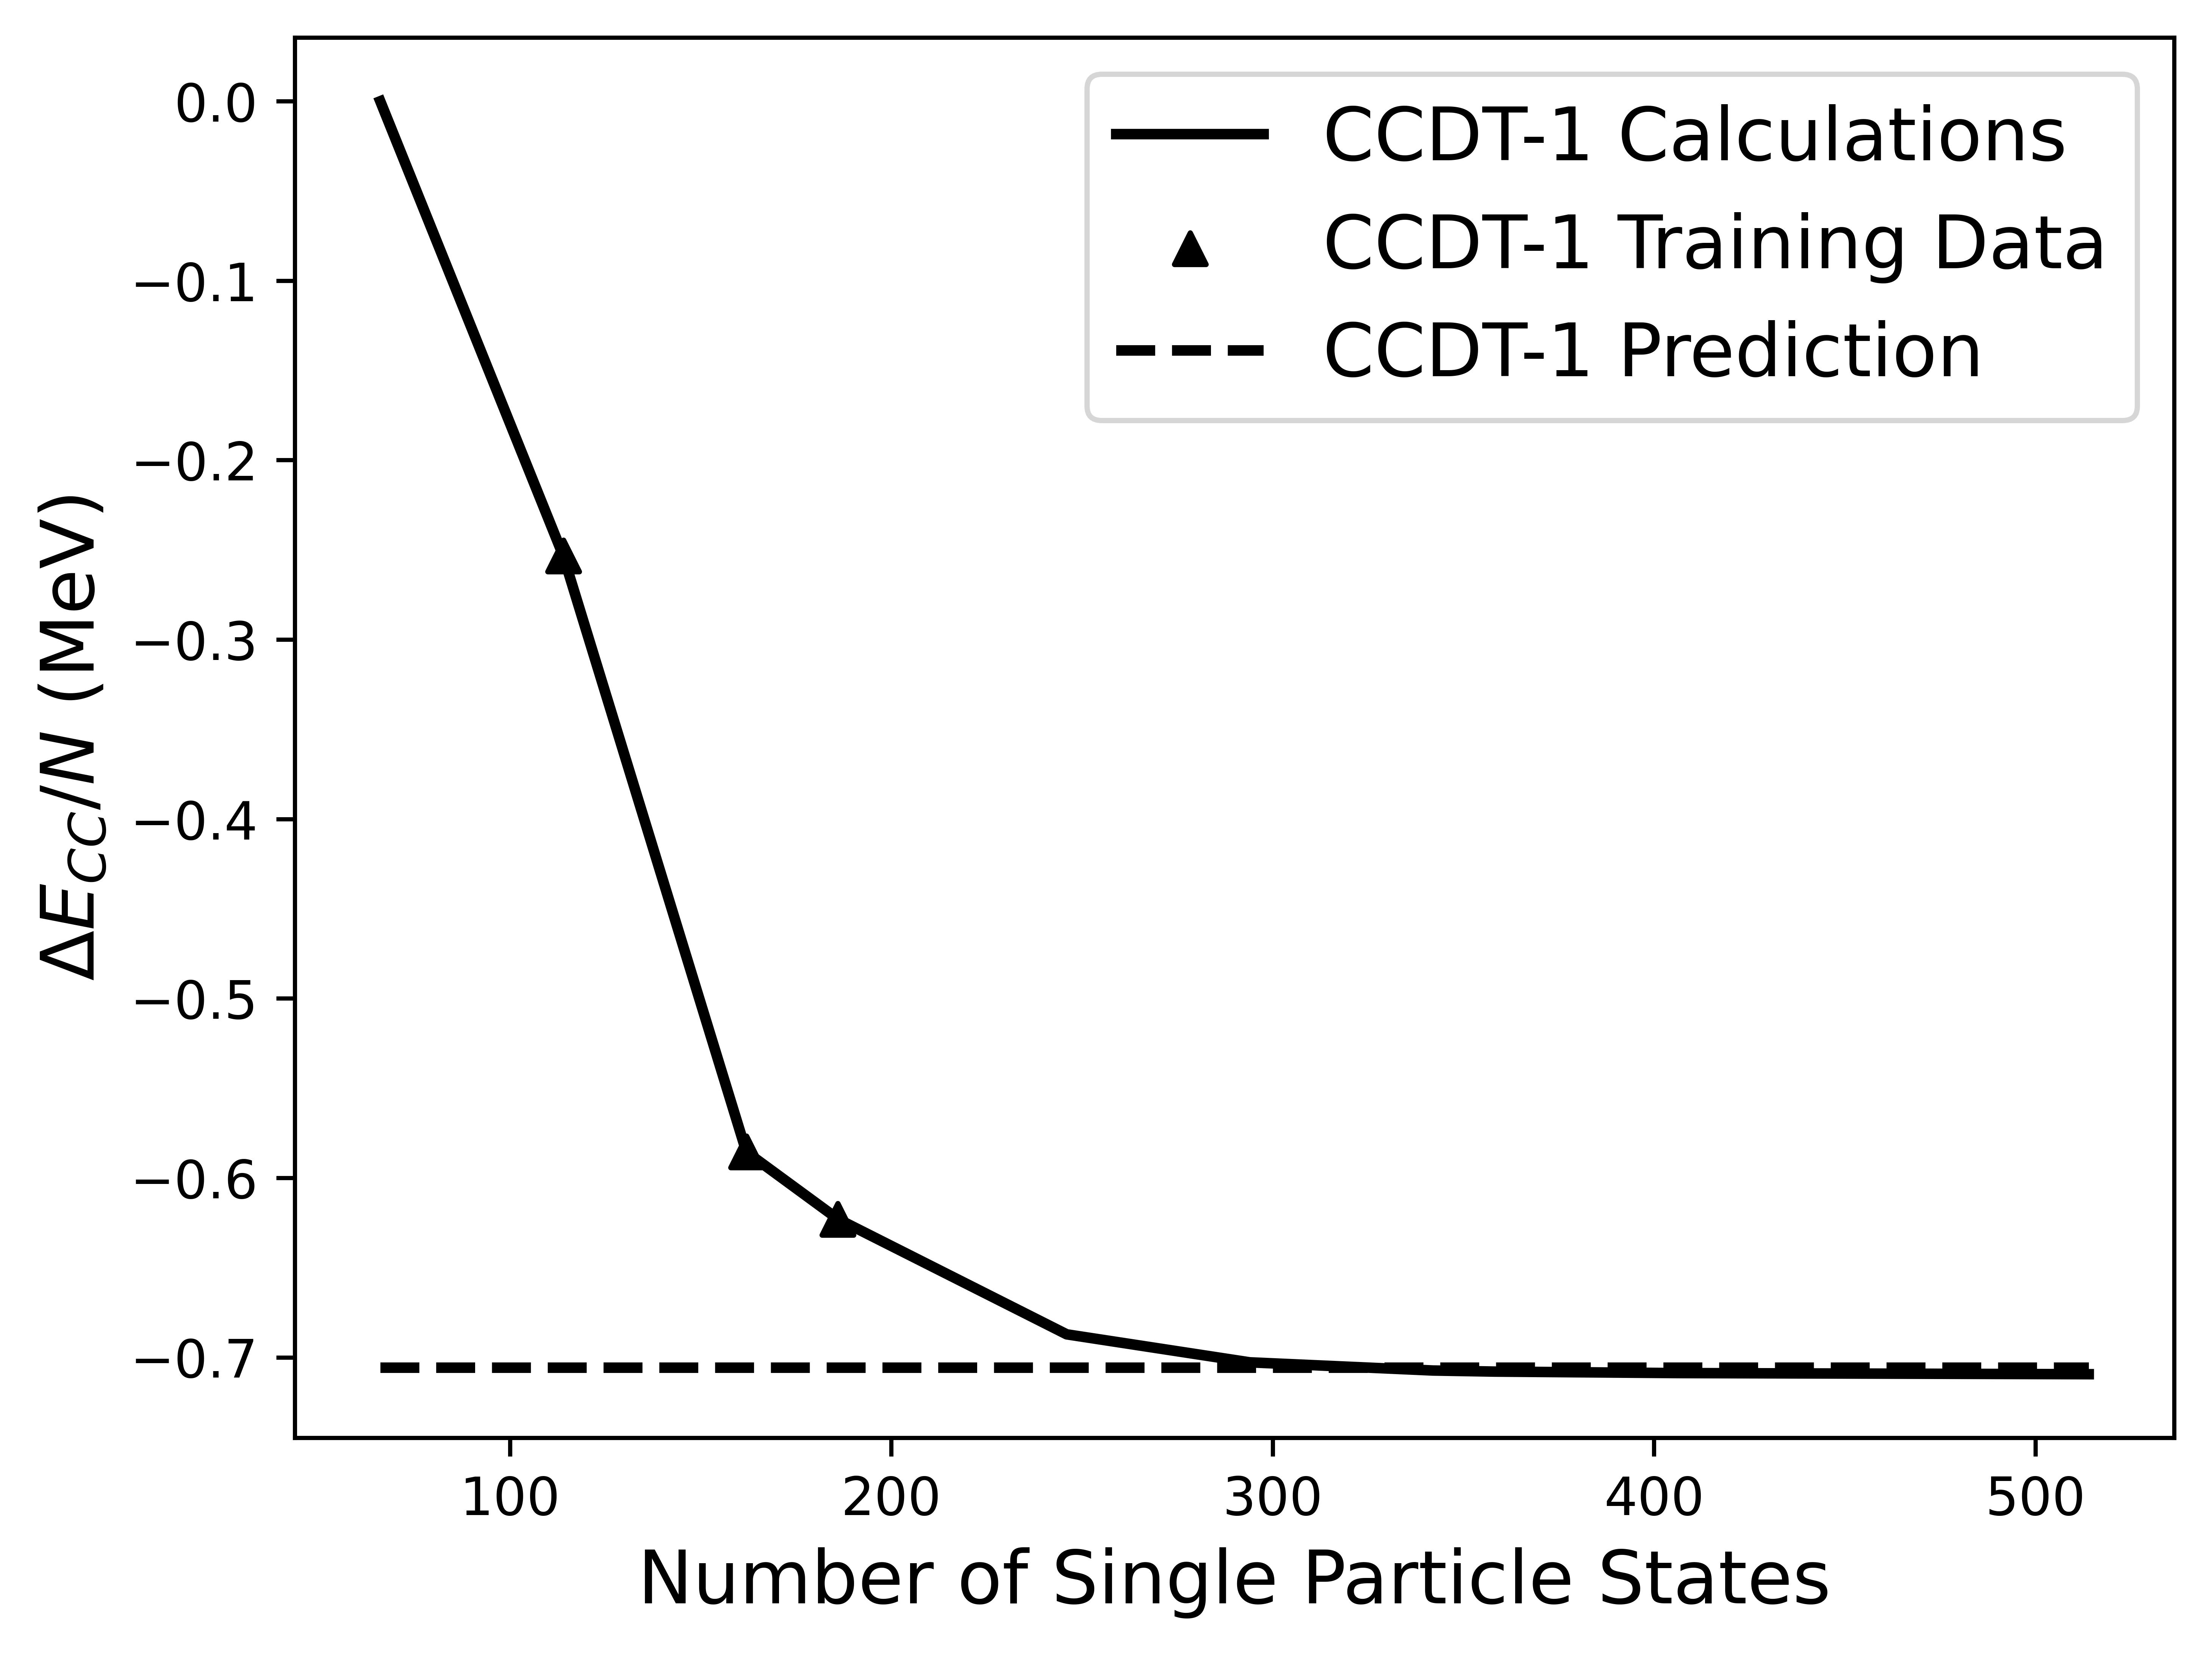
\includegraphics[scale=0.75]{Images/Chapter7/ORNL/CCDT1_Initial.png}
    \caption{The results performing coupled-cluster calculations with the CCDT-1 approximation on a pure neutron matter system with chiral NNLO potentials, 66 neutrons, and d = 0.16 fm$^{-3}$. The full calculations are shown with a solid line, the training data used for the SRE algorithm is shown with the triangular markers, and the SRE prediction for the converged correlation energy is shown with the dashed line. The percent error between the SRE prediction and the fully calculated converged correlation energy is 0.51$\%$, and the time savings for performing the SRE method is 180.68 node hours.}
    \label{fig:one_ccdt1_density}
\end{figure}

Now that we have shown that the SRE method can be feasibly applied to predict converged CCDT-1 correlation energies using only the MBPT2 energies, we can use this method to predict the correlation energies at various densities. Fig. \ref{fig:pnm_ccdt1_nuclear} compares the correlation energies from the last point in the training data at M = 186 (red dashed line), the fully calculated converged $\Delta E_{CCDT1}$ at 514 single-particle states (black line), and the SRE prediction for the converged correlation energies at densities around nuclear density. We can see that the training data is far from the converged values, and in fact, the difference between the M = 186 plot and the M = 514 plot is highest at the lower densities shown here. This is to show that the correlation energies used to train the SRE algorithm are not converged, and thus, a noticeable improvement is made over just using the training data. For Fig. \ref{fig:pnm_ccdt1_nuclear}, the average percent error between the SRE predictions and the complete calculations is 0.45$\%$. Furthermore, the total computational time saved when generating the six data points with the SRE method over fully generating them at 514 single-particle states is 917.30 node hours.

\begin{figure}
  \centering
  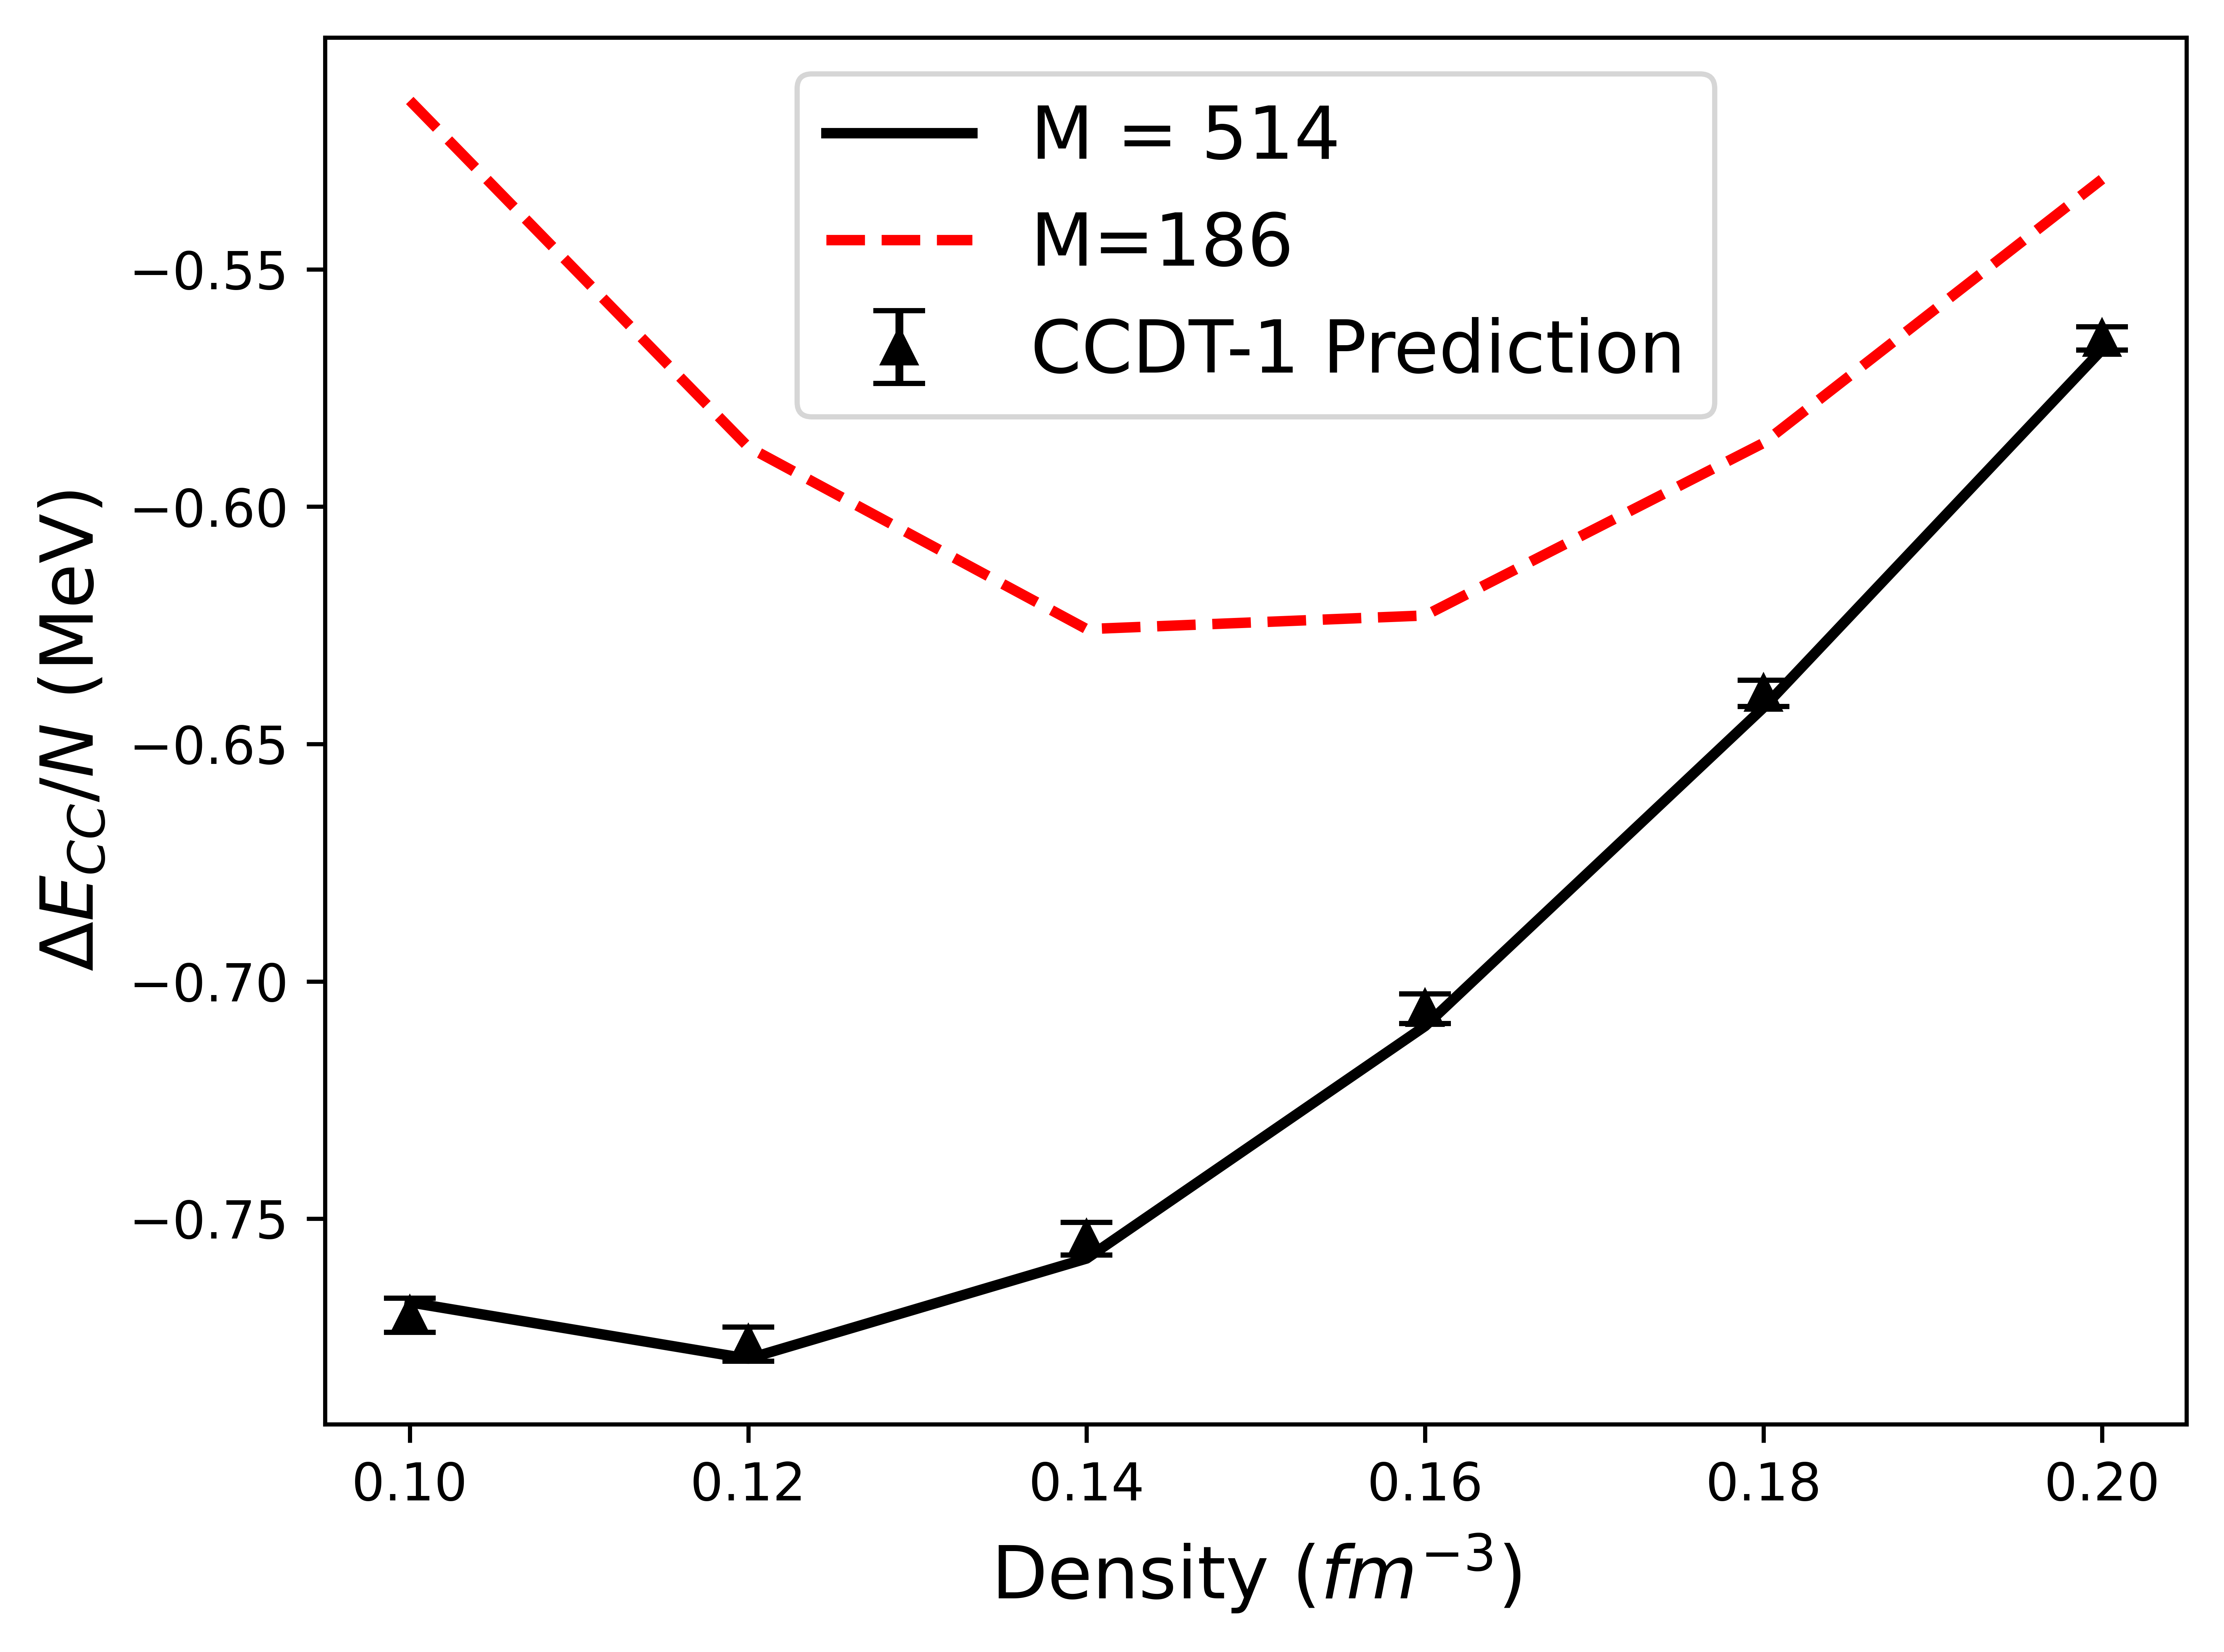
\includegraphics[scale=0.5]{Images/Chapter7/ORNL/ccdt1_nuclear_neutron_matter_with_training.png}
  \caption{The results from predicting the converged $\Delta E_{CCDT1}/N$ for pure neutron matter at densities around nuclear density.  The average percent error across all densities is 0.45$\%$, and the time savings from generating only the training data versus the fully converged $\Delta E_{CCDT1}/N$ is 917.30 node hours.}  \label{fig:ccdt1_nuclear_density}
\end{figure}

Finally, let us compare the CCDT-1 results to the CCD results for densities around nuclear density.

\begin{figure}
    \centering
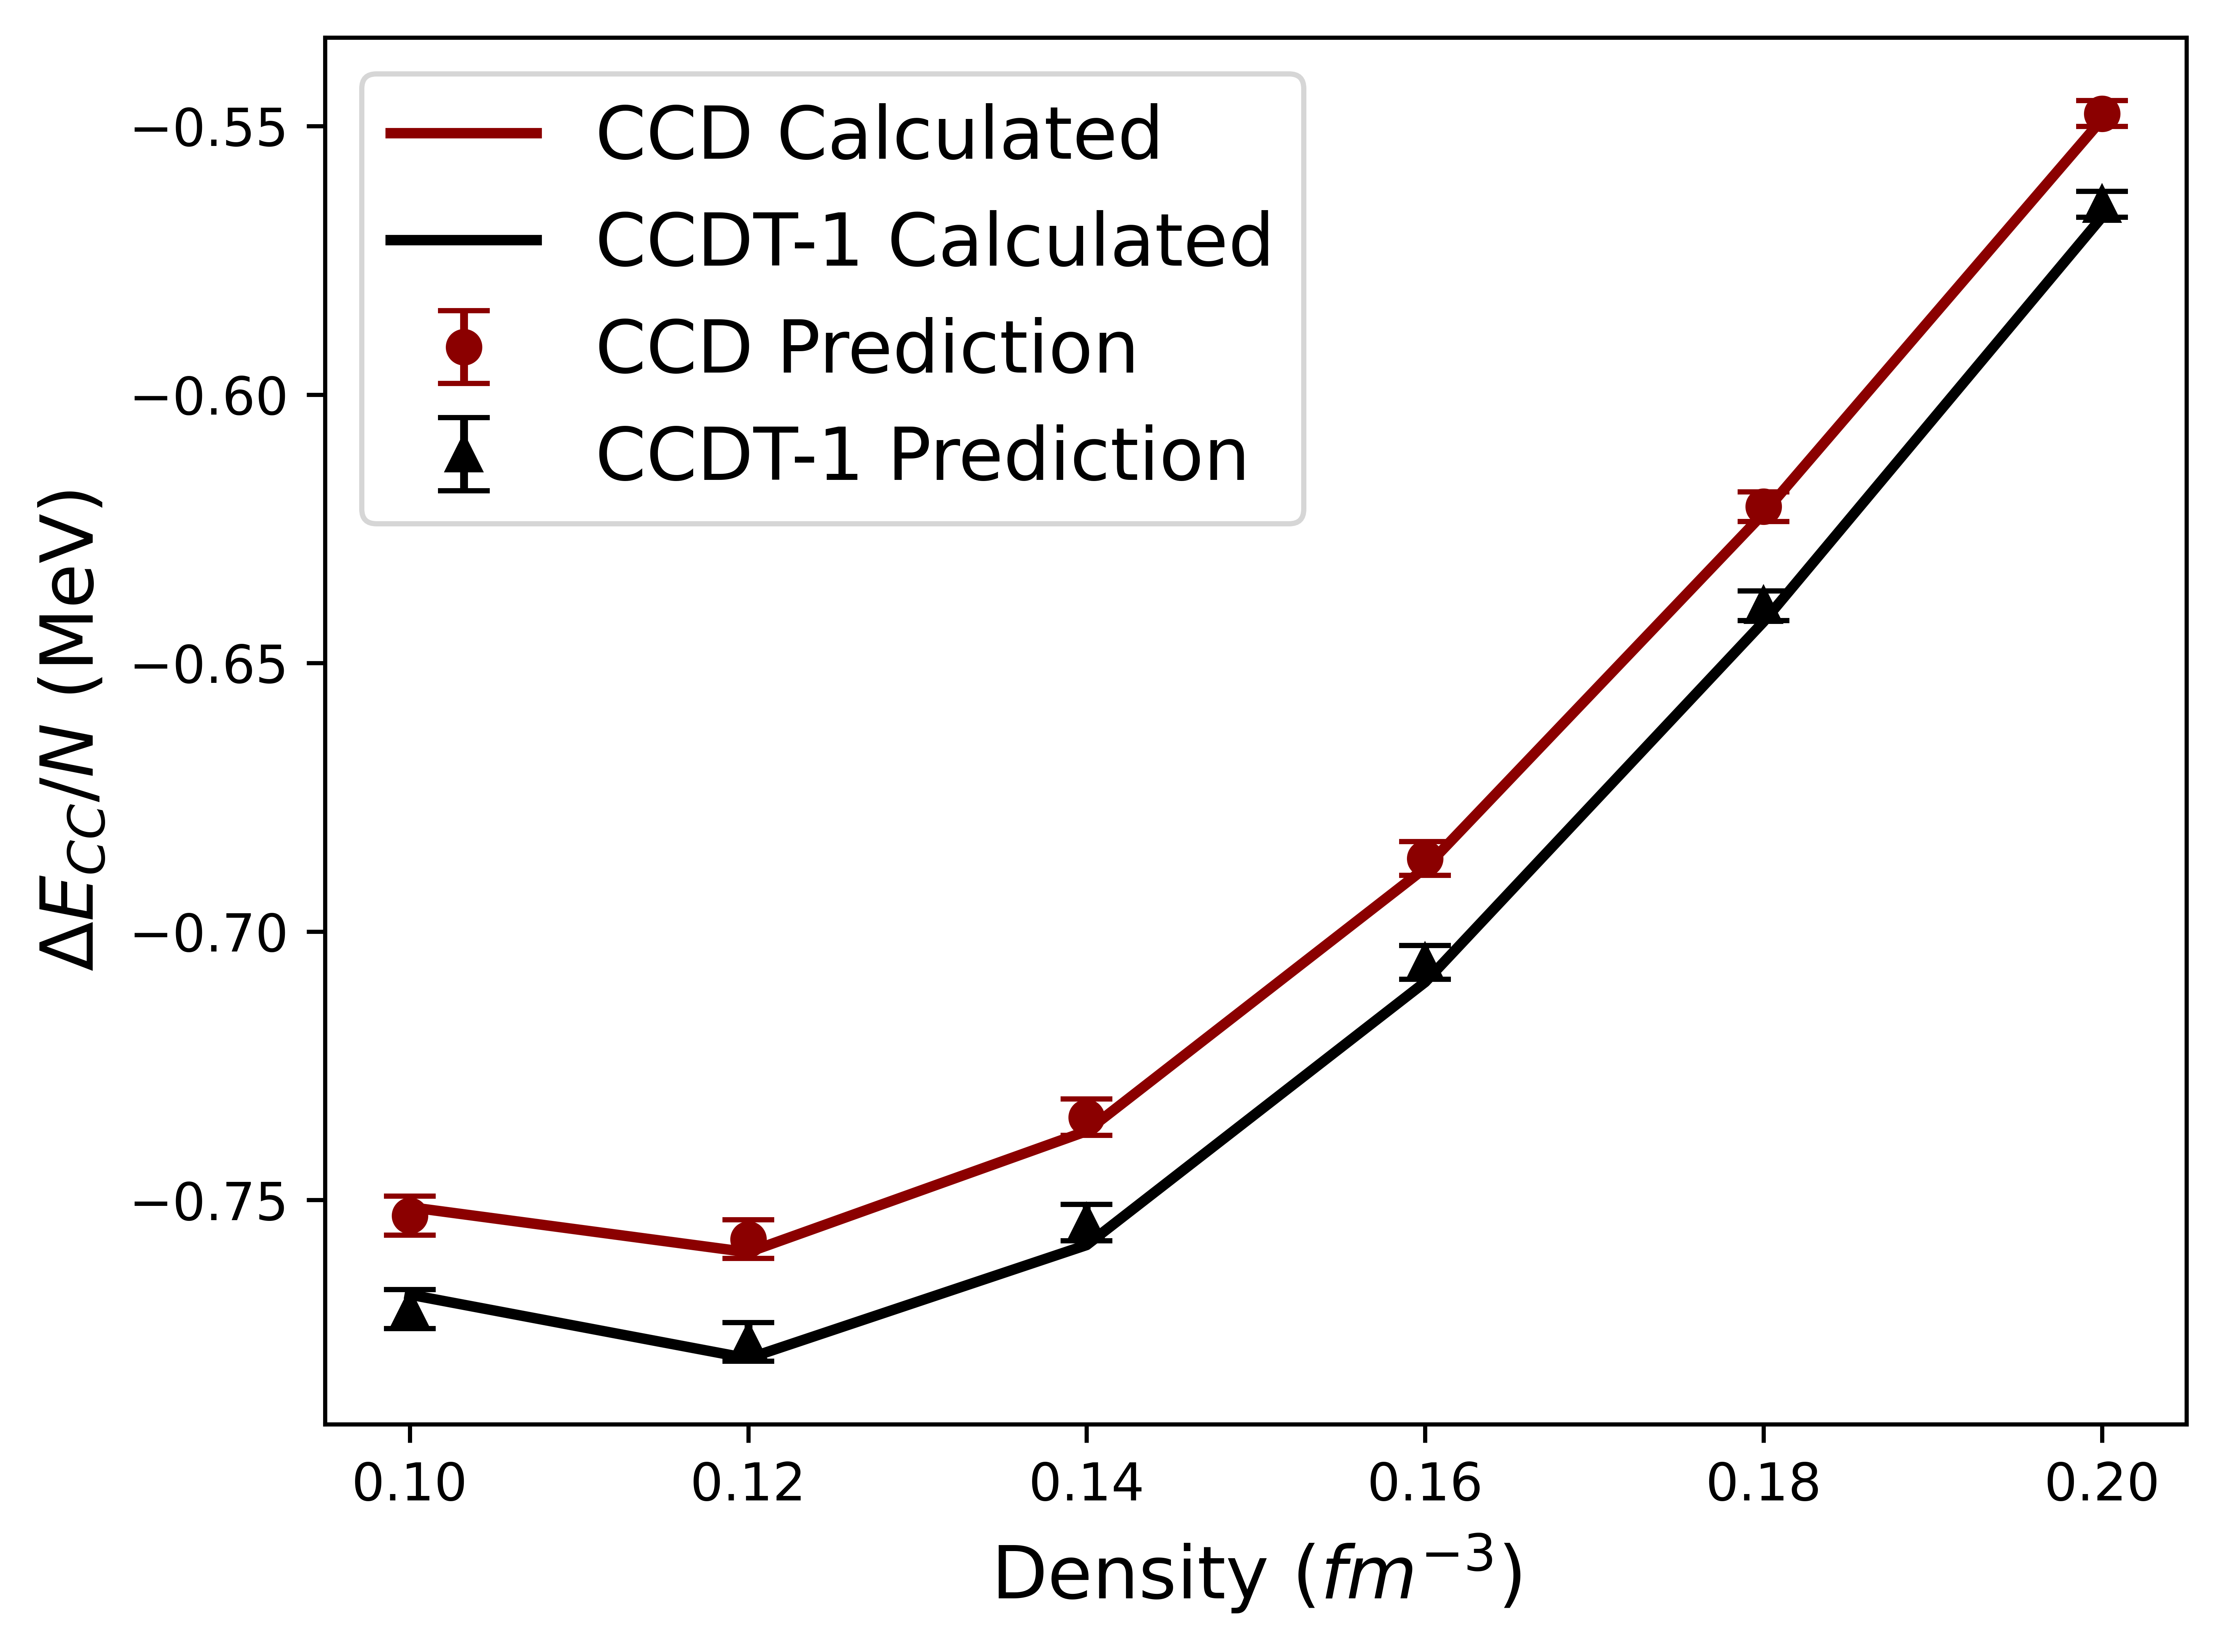
\includegraphics{Images/Chapter7/ORNL/ccdt1_nuclear_neutron_matter.png}
    \caption{CCD (red) versus CCDT-1 (black) correlation energies for a pure neutron matter system with 66 neutrons and chiral potentials. The converged correlation energies from full calculations are shown with solid lines, and the points represent the machine-learning predictions. The machine learning prediction is shown with the uncertainties from the Gaussian process algorithm.}
    \label{fig:ccd_and_ccddt1}
\end{figure}
